%-------------------------------------------------------------------------------------------------------
%-------------------------------------------------------------------------------------------------------
% Doc class

\documentclass[11pt,a4paper,twoside]{article}

%-------------------------------------------------------------------------------------------------------
%-------------------------------------------------------------------------------------------------------
% Define external packages, language, margins, fonts and new commands


\usepackage[utf8]{inputenc}
\usepackage[english]{babel}
\usepackage{notoccite}
\usepackage[skip=0.5\baselineskip]{caption}
\hyphenation{GTKWave}
\usepackage{listings}
\usepackage[all]{nowidow}

\usepackage{graphicx}
\graphicspath{ {./} {../../figlib/} }
\def\FontLn{% 16 pt normal
  \usefont{T1}{phv}{m}{n}\fontsize{16pt}{16pt}\selectfont}
\def\FontLb{% 16 pt bold
  \usefont{T1}{phv}{b}{n}\fontsize{16pt}{16pt}\selectfont}
\def\FontMn{% 14 pt normal
  \usefont{T1}{phv}{m}{n}\fontsize{14pt}{14pt}\selectfont}
\def\FontMb{% 12 pt bold
  \usefont{T1}{phv}{b}{n}\fontsize{12pt}{12pt}\selectfont}
\def\FontSn{% 12 pt normal
  \usefont{T1}{phv}{m}{n}\fontsize{12pt}{12pt}\selectfont}


\renewcommand{\rmdefault}{phv}
\renewcommand{\sfdefault}{phv}
\usepackage{geometry}	
\geometry{verbose,tmargin=2.5cm,bmargin=2.5cm,lmargin=2.5cm,rmargin=2.5cm}


\usepackage[pdftex]{hyperref} % enhance documents that are to be
                              % output as HTML and PDF
\hypersetup{colorlinks,       % color text of links and anchors,
                              % eliminates borders around links
%            linkcolor=red,    % color for normal internal links
            linkcolor=black,  % color for normal internal links
            anchorcolor=black,% color for anchor text
%            citecolor=green,  % color for bibliographical citations
            citecolor=black,  % color for bibliographical citations
%            filecolor=magenta,% color for URLs which open local files
            filecolor=black,  % color for URLs which open local files
%            menucolor=red,    % color for Acrobat menu items
            menucolor=black,  % color for Acrobat menu items
%            pagecolor=red,    % color for links to other pages
%            pagecolor=black,  % color for links to other pages
%            urlcolor=cyan,    % color for linked URLs
            urlcolor=black,   % color for linked URLs
	          bookmarks=true,         % create PDF bookmarks
	          bookmarksopen=false,    % don't expand bookmarks
	          bookmarksnumbered=true, % number bookmarks
	          pdftitle={report},
            pdfauthor={Andre C. Marta},
%            pdfsubject={Thesis Title},
%            pdfkeywords={Thesis Keywords},
            pdfstartview=FitV,
            pdfdisplaydoctitle=true}

% References in numbered list [1],[2],...
\usepackage[numbers,sort&compress]{natbib}
\usepackage{subcaption} 
\usepackage{mdframed}

%%%%%%%%%%%%%%%%%%%%%%%%%%%%%%%%%%%%%%%%%%%%%%%%%%%%%%%%%%%%%%%%%%%%%%%%
%     			    Begin Document                              %
%%%%%%%%%%%%%%%%%%%%%%%%%%%%%%%%%%%%%%%%%%%%%%%%%%%%%%%%%%%%%%%%%%%%%%%%


\begin{document}
\pagestyle{plain}


%-------------------------------------------------------------------------------------------------------
%-------------------------------------------------------------------------------------------------------
%  Cover page

%-------------------------------------------------------------------------------------------------------
%-------------------------------------------------------------------------------------------------------
% Page style

\thispagestyle {empty}

%-------------------------------------------------------------------------------------------------------
%-------------------------------------------------------------------------------------------------------
% IST logo

\begin{figure}[ht]
	\centering
	\includegraphics[width = 0.5\linewidth]{ist_foto}
\end{figure}

%-------------------------------------------------------------------------------------------------------
%-------------------------------------------------------------------------------------------------------
% Text/info

\begin{center}

	\vspace{2cm}
	{\FontLb Circuit Theory and Electronics Fundamentals} \\

	\vspace{0.5cm}
	{\FontSn Department of Electrical and Computer Engineering, Técnico, University of Lisbon} \\

	\vspace{0.5cm}
	{\FontSn April 5, 2021} \\

	\vspace{1cm}
	{\FontLb --------------------------------------------------------------------------------} \\
	\vspace{0.1cm}
	{\FontLb Laboratory Assignment - T4} \\
	{\FontLb --------------------------------------------------------------------------------} \\

	\vspace{1cm}
	{\FontMb Group nº59} \\
	\vspace{0.25cm}
	{\FontSn José Miguel Goulão - $95814$} \\
	{\FontSn Lourenço Pacheco - $95817$} \\
	{\FontSn André Gomes - $96352$} \\

	\vspace{.5cm}

\end{center}




%-------------------------------------------------------------------------------------------------------
%-------------------------------------------------------------------------------------------------------
% Contents & Body

\tableofcontents

	\vspace{2cm}
	%-------------------------------------------------------------------------------------------------------
%-------------------------------------------------------------------------------------------------------
% Sec & Label

\section{Introduction}
\label{sec:introduction}

%-------------------------------------------------------------------------------------------------------
%-------------------------------------------------------------------------------------------------------


The objective of this laboratory assignment is to optimize and study an AC/DC converter
circuit. We were given total freedom to choose the architecture of the Envelope Detector
and Voltage Regulator circuits. Our goal is to achieve the highest merit($M$) possibe. This
value is obtained with the following equations:
	
\[
M = \frac{1}{cost\times (Ripple(vout) + avg(vout-12) + 10^{-6})}
\]

\[
 cost = cost_{resistors} + cost_{capacitor} + cost_{diodes} 
\]

$cost_{resistors} = 1MU/kOhm$; $cost_{capacitors} = 1MU/\mu- F$;
$cost_{diodes} = 0.1MU/diode$ \\

For reasons explained later, our circuit (in total) contains:

\begin{itemize}
	\item one voltage source ($V_1$)
	\item two inductors ($L_1$,$L_2$)
	\item one resistor ($R_1$)
	\item one capacitor ($C_1$)
	\item twenty diodes ($D_1$-$D_{20}$)
\end{itemize}

In Section \ref{sec:analysis}, a theoretical analysis of the circuit is presented. In
Section \ref{sec:simulation} , the circuit is analysed by simulation, and the results are
compared to the theoretical results obtained in Section \ref{sec:analysis}. The conclusions
of this study are outlined in Section \ref{sec:conclusion}.


\begin{figure}[h]
	\centering
	\includegraphics[width=0.85\linewidth]{dsnh_t3.pdf}
	\caption{Circuit T3}
\label{fig:Desenho_t3}
\end{figure}




	\vspace{2cm}
	%-------------------------------------------------------------------------------------------------------
%-------------------------------------------------------------------------------------------------------
% Sec & Label

\section{Theoretical Analysis}
\label{sec:analysis}


%-------------------------------------------------------------------------------------------------------
%-------------------------------------------------------------------------------------------------------
% Intro

In this section, the Circuit T2 is analysed theoretically. In figure \ref{fig:Dsnh_oct_t2},
appart from all the components being identified, the assumed currents are also shown.
Only the node method was used in this section. Each subsection refers to each task.


Three important equations were used: both Kirchhoff's laws (Kirchhof's current law (KCL)
- eq.(\ref{eq:kcl}) and Kirchhoff's voltage law (KVL) - eq.(\ref{eq:kvl})); Ohm's law
(eq.(\ref{eq:ohm})).

The algebraic sum of all the currents in any given node is zero:
\begin{equation}
	\sum I_i = 0
	\label{eq:kcl}
\end{equation}

The algebraic sum of all the voltages in any given closed-loop circuit (mesh) is zero:
\begin{equation}
	\sum V_i = 0
	\label{eq:kvl}
\end{equation}

The potential difference between the two nodes connected to a resistor is equal to the current that 
passes through the resistor multiplied by its resistance.
\begin{equation}
	V_i = R_iI_i
	\label{eq:ohm}
\end{equation}

\begin{equation}
	V_1(t) = V_2(\infty) + [V_2(0) - V_2(\infty)]e^{\frac{-t}{\tau}}
\end{equation}

\newpage

%-----------------------------------------------------------------------
%-----------------------------------------------------------------------
% 			      task1 - subsec
% ----------------------------------------------------------------------
% ----------------------------------------------------------------------
\subsection{Task 1)}
\label{subsec:task1_a}

\begin{figure}[ht]
	\centering
	\includegraphics[width=0.75\linewidth]{dsnh_oct_t2_al1.pdf}
	\caption{Circuit T2 when $t<0$}
\label{fig:Dsnh_sim_t2}
\end{figure}

When $t<0$ the value of $V_s$ is constant and so we can perform DC analysis on the circuit. We can assume that enough time has passed and so it is reasonable to assume that the circuit is in steady-state.

When performing a DC steady-state analysis on a circuit we can use the fact that the current flowing trough the capacitor is null (the circuit behaves as if the capacitor was removed).

A node analysis was performed to find the voltage value of each node and the current in each branch.

The node method uses KCL in conjunction with Ohm’s law to define equations that when solved give the voltage value 
of each nove in relation to ground (Node 4, $V_4 = 0$). 

In order to have equations that solve for the node’s voltage, a relation between curent and voltage is made using 
Ohm’s law (given a resistance between two nodes, the current that passes the resistance can be written as 
$I=\frac{V_2-V_1}{R_1}$)

To simplify the equations it is useful to use the conductance $G_n$ which is the inverse of the resistance $R_n$ 
($G_n=\frac{1}{R_n}$)

The equations used to solve the circuit were organized in matrix form.

{\footnotesize

$ \begin{bmatrix}
1 & 0 & 0 & 0 & 0 & 0 & 0 & 0 & 0 & 0 \\
G1 & -(G1+G2+G3) & G2 & G3 & 0 & 0 & 0 & 0 & 0 & 0 \\
0 & -G2 & G2 & 0 & 0 & 0 & 0 & 0 & -1 & 0 \\
0 & G3 & 0 & -(G3+G4+G5) & G5 & 0 & 0 & 0 & 0 & 0 \\
0 & 0 & 0 & -G5 & G5 & 0 & 0 & 0 & 1 & 1 \\
0 & 0 & 0 & 0 & 0 & G7 & -G7 & -1 & 0 & 1 \\
0 & 0 & 0 & 0 & 0 & -(G6+G7) & G7 & 0 & 0 & 0 \\
0 & 0 & 0 & 0 & 0 & 0 & 0 & 0 & 0 & 1 \\
0 & 0 & 0 & 1 & 0 & G6*K_d & -1 & 0 & 0 & 0 \\
0 & K_b & 0 & -K_b & 0 & 0 & 0 & 0 & -1 & 0 
\end{bmatrix}  $
$ \begin{bmatrix}
V1 \\
V2 \\
V3 \\
V5 \\
V6 \\
V7 \\
V8 \\
IH1 \\
Ib \\
Ic \\
\end{bmatrix}  $
=
$ \begin{bmatrix}
Vs\\
0\\
0\\
0\\
0\\
0\\
0\\
0\\
0\\
0\\
\end{bmatrix}  $
}

Figure \ref{fig:Desenho_t2}. In adition, assume $V_{Ni}$ to be the voltage in node $Ni$ (every node position can
also be found in Figure \ref{fig:Desenho_t2}). \\

\begin{table}[H]
	\centering
	\begin{tabular}{|l|r|}
    		\hline    
    		{\bf Name} & {\bf Value [A or V]} \\ \hline
    		$V_{N1}$ & 5.114025e+00 \\ \hline 
$V_{N2}$ & 4.830792e+00 \\ \hline 
$V_{N3}$ & 4.226624e+00 \\ \hline 
$V_{N5}$ & 4.871651e+00 \\ \hline 
$V_{N6}$ & 5.781844e+00 \\ \hline 
$V_{N7}$ & -1.849204e+00 \\ \hline 
$V_{N8}$ & -2.786253e+00 \\ \hline 
$@I_{b}$ & -2.957272e-04 \\ \hline 
$@I_{c}$ & 0.000000e+00 \\ \hline 
$@I_{d}$ & -9.187358e-04 \\ \hline 
$@I_{H1}$ & 9.187358e-04 \\ \hline 

  	\end{tabular}
  	\caption{Values computed by Octave. Variables identified with a '$@$' have a
  	corresponding value in Ampere (A). The others are expressed in Volts (V).}
 
\label{tab:node}
\end{table}
\newpage
%-----------------------------------------------------------------------
%-----------------------------------------------------------------------
% 			      task2 - subsec
% ----------------------------------------------------------------------
% ----------------------------------------------------------------------
\subsection{Task 2)}
\label{subsec:task2_a}

\begin{figure}[H]
	\centering
	\includegraphics[width=0.75\linewidth]{dsnh_oct_t2_al2.pdf}
	\caption{Circuit T2 at $t=0$}
\label{fig:Dsnh_sim_t2}
\end{figure}

In this section the capacitor is replaced with a voltage source $V_x$ with value $V_x = V_6 - V_8$ as shown in figure.... The same type of analysis was made to this circuit but with a slightly modification on some of the rows to represent the modified circuit.

{\footnotesize

$ \begin{bmatrix}
1 & 0 & 0 & 0 & 0 & 0 & 0 & 0 & 0 & 0 \\
G1 & -(G1+G2+G3) & G2 & G3 & 0 & 0 & 0 & 0 & 0 & 0 \\
0 & -G2 & G2 & 0 & 0 & 0 & 0 & 0 & -1 & 0 \\
0 & G3 & 0 & -(G3+G4+G5) & G5 & 0 & 0 & 0 & 0 & 0 \\
0 & 0 & 0 & -G5 & G5 & 0 & 0 & 0 & 1 & 1 \\
0 & 0 & 0 & 0 & 0 & G7 & -G7 & -1 & 0 & 1 \\
0 & 0 & 0 & 0 & 0 & -(G6+G7) & G7 & 0 & 0 & 0 \\
0 & 0 & 0 & 0 & 1 & 0 & -1 & 0 & 0 & 0 \\
0 & 0 & 0 & 1 & 0 & G6*K_d & -1 & 0 & 0 & 0 \\
0 & Kb & 0 & -K_b & 0 & 0 & 0 & 0 & -1 & 0 
\end{bmatrix}  $
$ \begin{bmatrix}
V1 \\
V2 \\
V3 \\
V5 \\
V6 \\
V7 \\
V8 \\
IH1_2 \\
Ib_2 \\
Ic_2 \\
\end{bmatrix}  $
=
$ \begin{bmatrix}
0 \\
0 \\
0 \\
0 \\
0 \\
0 \\
0 \\
Vx \\
0 \\
0 \\
\end{bmatrix}  $
}


\begin{table}[ht]
	\centering
	\begin{tabular}{|l|r|}
    		\hline    
    		{\bf Name} & {\bf Value [A or V]} \\ \hline
    		$V_{N1}$ & 0.000000e+00 \\ \hline 
$V_{N2}$ & -7.143971e-16 \\ \hline 
$V_{N3}$ & -2.238283e-15 \\ \hline 
$V_{N5}$ & -6.113379e-16 \\ \hline 
$V_{N6}$ & 8.568097e+00 \\ \hline 
$V_{N7}$ & 1.476238e-16 \\ \hline 
$V_{N8}$ & -0.000000e+00 \\ \hline 
$@I_{b}$ & -7.459097e-19 \\ \hline 
$@I_{d}$ & 7.334357e-20 \\ \hline 
$@I_{H1}$ & -2.783827e-03 \\ \hline 
$@V_{x}$ & 8.568097e+00 \\ \hline 
$@I_{x}$ & -2.783827e-03 \\ \hline 
$R_{eq}$ & 3.077812e+03 \\ \hline 
$\tau$ & 3.197736e-03 \\ \hline 

  	\end{tabular}
  	\caption{Values computed by Octave. Variables identified with a '$@$' have a
  	corresponding value in Ampere (A). The others are expressed in Volts (V), Ohm and time (s).}
 
\label{tab:node}
\end{table}


By performing this analysis we can compute the current $I_x$ that flows trough $V_s$. Using Ohm's law we can calculate the equivente resistance $R_{eq}$:

\[
R_{eq}=\frac{V_x}{I_x}
\]


This procedure is important to compute the circuit's time constant $\tau$ by using the equation $\tau = CR_{eq}$. The time constant in conjunction with the boundary conditions of the circuit are required to compute the natural solution of the circuit.



\newpage
%-----------------------------------------------------------------------
%-----------------------------------------------------------------------
% 			      task3 - subsec
% ----------------------------------------------------------------------
% ----------------------------------------------------------------------
\subsection{Task 3)}
\label{subsec:task3_a}

\begin{figure}[H]
	\centering
	\includegraphics[width=0.75\linewidth]{dsnh_oct_t2_al3.pdf}
	\caption{Circuit T2, natural response}
\label{fig:Dsnh_sim_t2}
\end{figure}

With the circuit's time constant $\tau$ and boundary conditions calculated in the previous task we can use following equation to get the natural solution of the circuit:

\[
V_{6n}(t) = V_6(\infty) + [V_6(0) - V_6(\infty)]e^{\frac{-t}{\tau}}
\] 

Since $V_s$ is considered to be null on this circuit, the value of node 6 is 0 at infinity $V_6(\infty) = 0$ 



\begin{figure}[H]
	\centering
	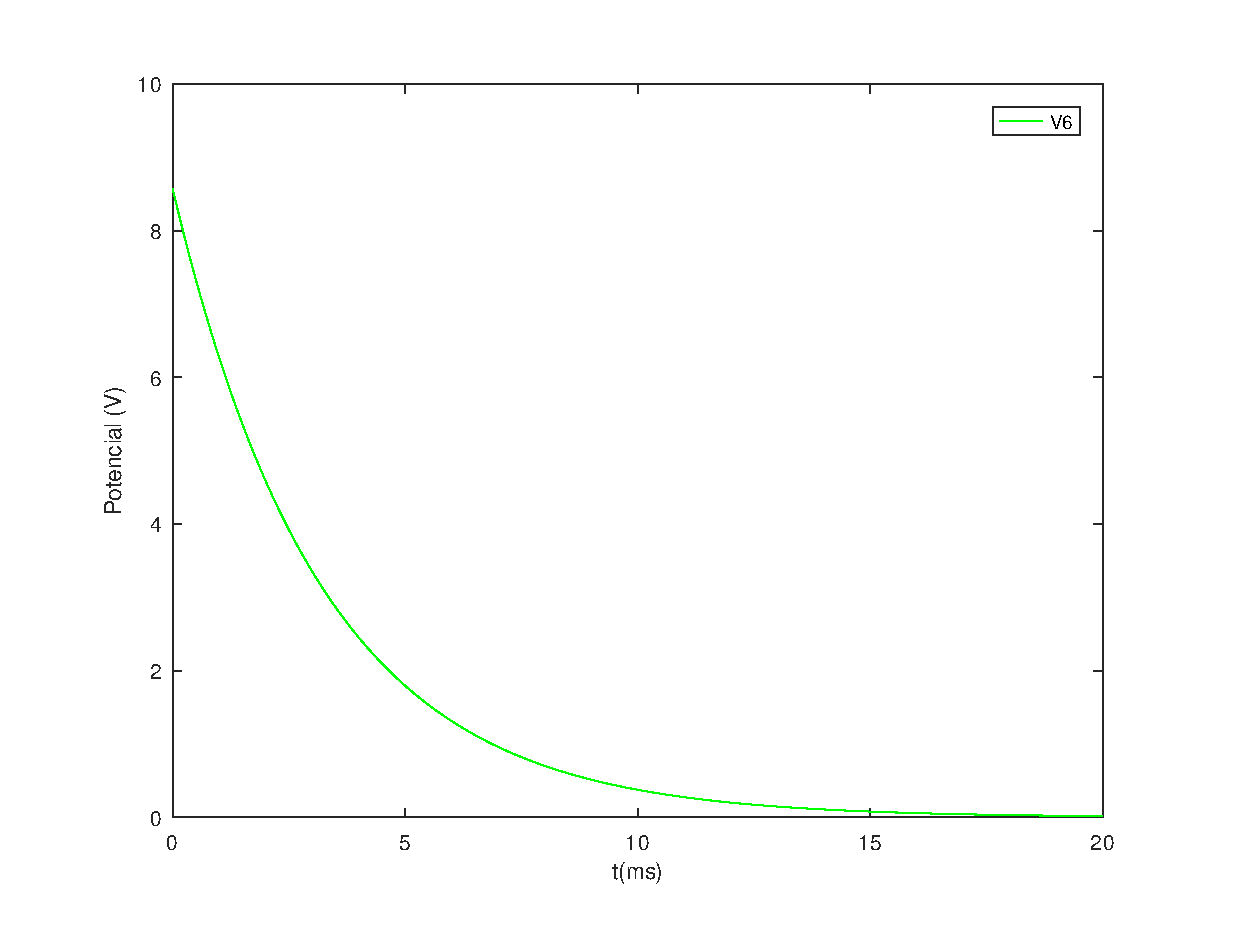
\includegraphics[width=0.8\linewidth]{plot1.eps}
	\caption{Natural response}
\label{fig:Dsnh_sim_t2}
\end{figure}


%-----------------------------------------------------------------------
%-----------------------------------------------------------------------
% 			      task4 - subsec
% ----------------------------------------------------------------------
% ----------------------------------------------------------------------
\subsection{Task 4)}
\label{subsec:task4_a}

\begin{figure}[H]
	\centering
	\includegraphics[width=0.75\linewidth]{dsnh_oct_t2_al456.pdf}
	\caption{Circuit T2}
\label{fig:Dsnh_sim_t2}
\end{figure}
\newpage

In this task the forced solution of the circuit is computed. To acomplish this objetive, we do an analysis using a phasor voltage source $V_s=1$ and replacing C with its impedance:

\[
Z_c = j\frac{1}{C\omega}
\]

Doing an analysis similar to the previous ones, with a slightly modified matrix we can determine the phasor voltages in all nodes.

{\footnotesize
$ \begin{bmatrix}
1 & 0 & 0 & 0 & 0 & 0 & 0 & 0 & 0 & 0 \\
G1 & -(G1+G2+G3) & G2 & G3 & 0 & 0 & 0 & 0 & 0 & 0 \\
0 & -G2 & G2 & 0 & 0 & 0 & 0 & 0 & -1 & 0 \\
0 & G3 & 0 & -(G3+G4+G5) & G5 & 0 & 0 & 0 & 0 & 0 \\
0 & 0 & 0 & -G5 & G5 & 0 & 0 & 0 & 1 & 1 \\
0 & 0 & 0 & 0 & 0 & G7 & -G7 & -1 & 0 & 1 \\
0 & 0 & 0 & 0 & 0 & -(G6+G7) & G7 & 0 & 0 & 0 \\
0 & 0 & 0 & 0 & -1/Z_c & 0 & 1/Z_c & 0 & 0 & 0 \\
0 & 0 & 0 & 1 & 0 & G6*K_d & -1 & 0 & 0 & 0 \\
0 & K_b & 0 & -K_b & 0 & 0 & 0 & 0 & -1 & 0 
\end{bmatrix}  $
$ \begin{bmatrix}
V1 \\
V2 \\
V3 \\
V5 \\
V6 \\
V7 \\
V8 \\
IH1 \\
Ib\\
Ic\\
\end{bmatrix}  $
=
$ \begin{bmatrix}
1 \\
0 \\
0 \\
0 \\
0 \\
0 \\
0 \\
0 \\
0 \\
0 \\
\end{bmatrix}  $

}

The following table shows the phasor magnitudes in each node.

\begin{table}[ht]
	\centering
	\begin{tabular}{|l|r|}
    		\hline    
    		{\bf Name} & {\bf Value [V]} \\ \hline
    		$V_{N1}$ & 1.000000e+00 \\ \hline 
$V_{N2}$ & 9.446163e-01 \\ \hline 
$V_{N3}$ & 8.264770e-01 \\ \hline 
$V_{N5}$ & 9.526060e-01 \\ \hline 
$V_{N6}$ & 5.470469e-01 \\ \hline 
$V_{N7}$ & 3.615947e-01 \\ \hline 
$V_{N8}$ & 5.448259e-01 \\ \hline 

  	\end{tabular}
  	\caption{Values computed by Octave.}
 
\label{tab:node}
\end{table}


%-----------------------------------------------------------------------
%-----------------------------------------------------------------------
% 			      task5 - subsec
% ----------------------------------------------------------------------
% ----------------------------------------------------------------------
\subsection{Task 5)}
\label{subsec:task5_a}

In this task we compute the final total solution $v_6(t)$ with a frequency of 1000Hz. To achieve the final result the phasors are converted to real time functions and than superimposed with the natural solution found before.

The force solution will have the form:

\[
V_{6f}(t) = V*sin(\omega t + \phi)
\]

The constant $\omega$ is the angular frequency of the voltage source, $V$ is the amplitude of the node phasor and $\phi$ is the phase shift of the node phasor.

The final solution will have the form:

\[
V_6(t) = V_{6n} + V_{6f}
\]

The following graph plots the results computed by octave in interval [-5, 20]ms.

\begin{figure}[ht]
	\centering
	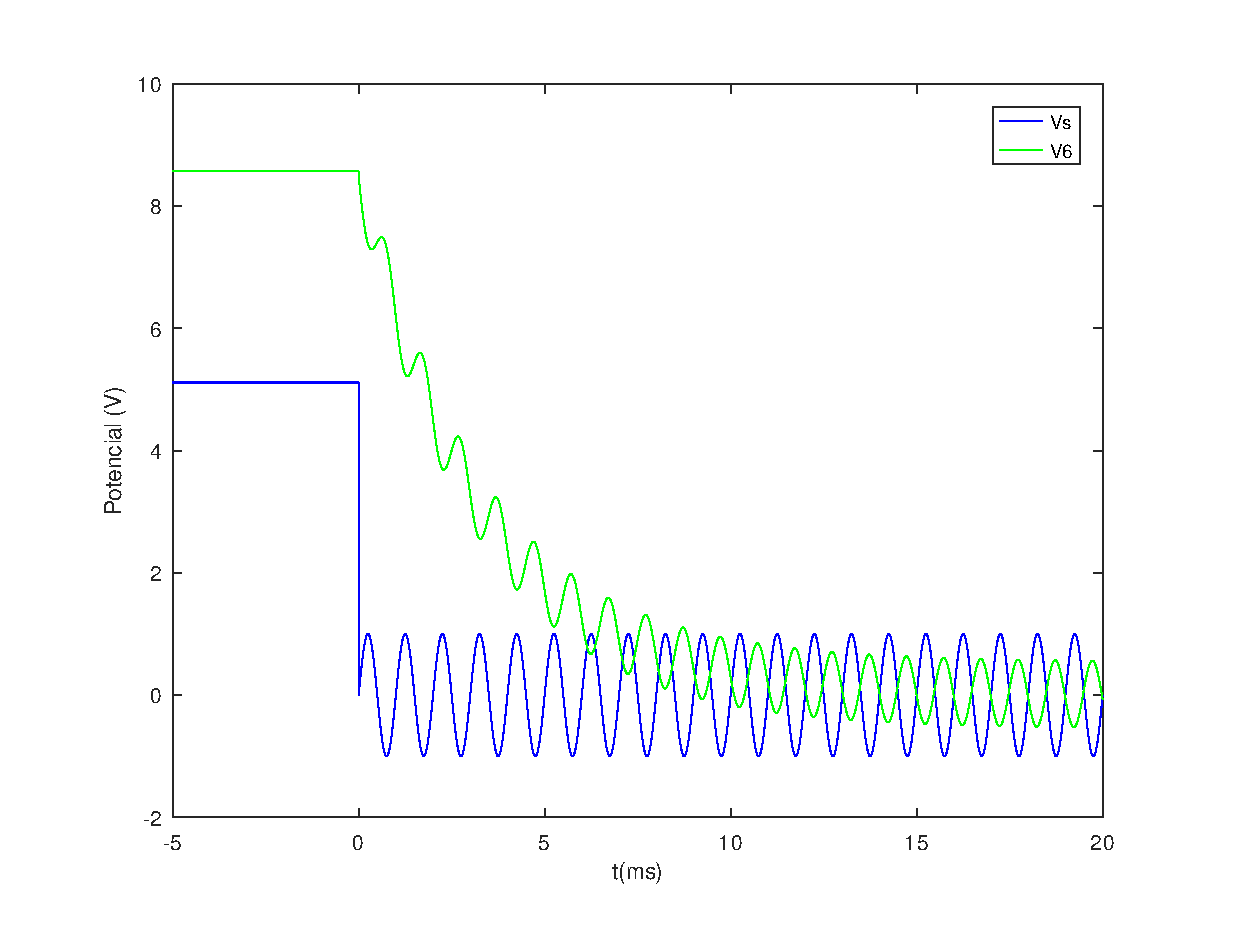
\includegraphics[width=0.8\linewidth]{plot2.eps}
	\caption{Final total response at 1kHz}
\label{fig:Dsnh_sim_t2}
\end{figure}
\newpage
%-----------------------------------------------------------------------
%-----------------------------------------------------------------------
% 			      task6 - subsec
% ----------------------------------------------------------------------
% ----------------------------------------------------------------------
\subsection{Task 6)}
\label{subsec:task6_a}

In this task, the frequency response of $v_c(f)= v_6(f) - v_8(f)$ and $v_6(f)$ is determined for a frequency range of 0.1Hz to 1 MHz. For the calculation of the frequecy response a similar analysis to the one in task 4) was made for a multitude of frequencys in the set the frequency range. The following graph shows the achieved results: 


\begin{figure}[ht]
	\centering
	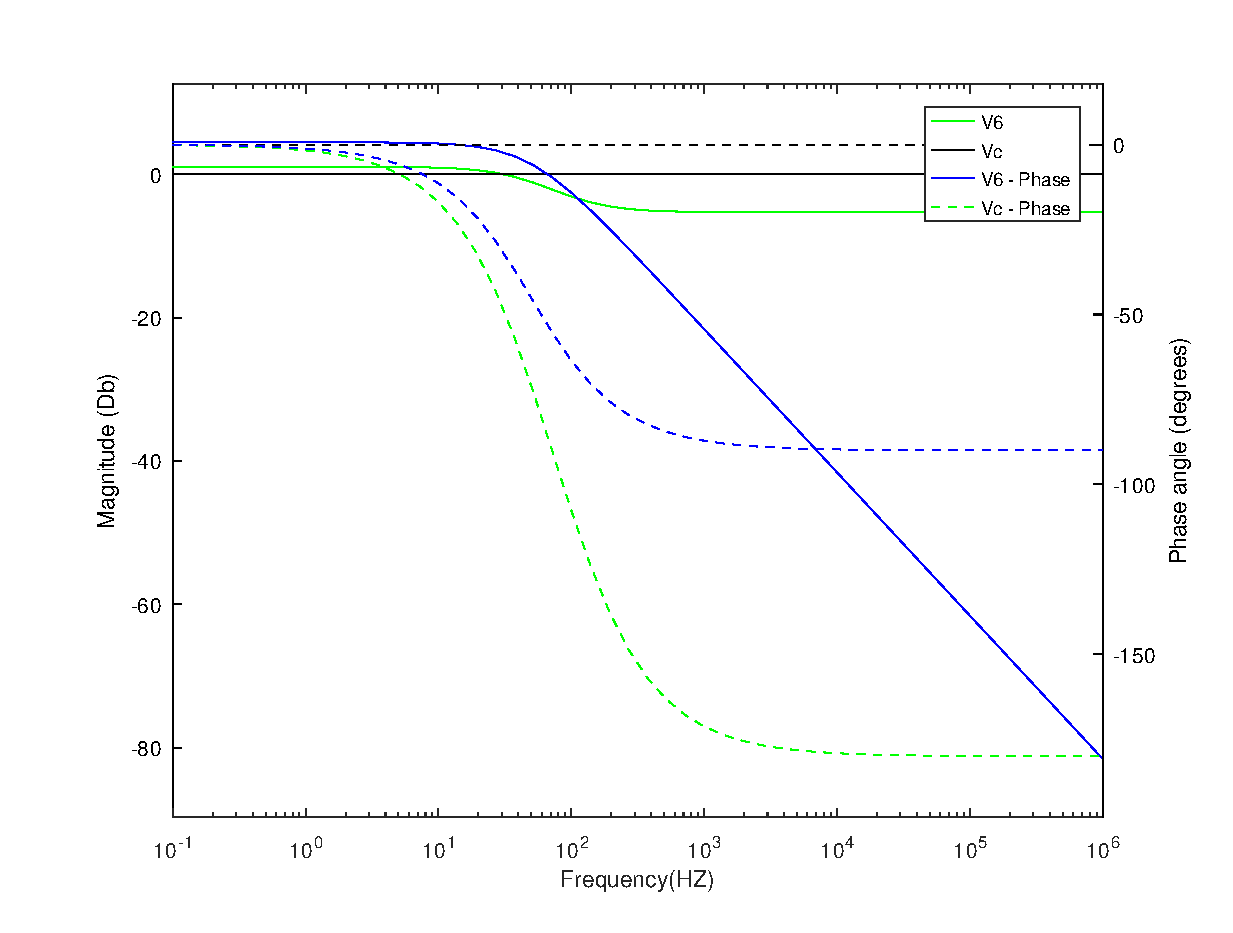
\includegraphics[width=0.9\linewidth]{plot3.eps}
	\caption{Frequency response analysis}
\label{fig:Dsnh_sim_t2}
\end{figure}

We can see that the value of $v_c(f)$ in dB decreases with increasing frequency. This behaviour is due to the impedance of the capacitor decreasing with larger frequencies and so the phasor voltage difference tends to zero (since the magnitude is ploted in dB, when a voltage approaches 0 the dB values goes to negative values).

The value of $v_c(f)$ also decreases for the same reasons explained in subsection 2.5).








	%-------------------------------------------------------------------------------------------------------
%-------------------------------------------------------------------------------------------------------
% Sec & Label

\section{Simulation Analysis}
\label{sec:simulation}


%-------------------------------------------------------------------------------------------------------
%-------------------------------------------------------------------------------------------------------
% Intro

In this section, Circuit T1 is reproduced with the help of Ngspice.

Firstly, the outcome of the simulation is shown, as well as a brief explanation
on how it was achived. Afterwards, a comparison is done between those values and
the ones attained in Section \ref{sec:analysis}.



%-----------------------------------------------------------------------
%-----------------------------------------------------------------------
% 			     Results - subsec
% ----------------------------------------------------------------------
% ----------------------------------------------------------------------

\subsection{Simulated results}
\label{subsec:sim_res}


% ----------------------------------------------------------------------
% Text

Ngspice is a simulator for eletronic circuits that can output a variety of results.
This emulator computes the voltages in every node, as well as the potential difference
between two given nodes. Apart from that, the group made use of the command
{\em .options savecurrents} which also enables the output of the currents that pass
through all branches.

With the limitation that Ngspice only provides the current in the components and not through
the nodes, an aditional voltage source ($Vaux$) was added so that the current in $R_6$ ($I_c$)
is known. This source (not displayed in Figure \ref{fig:Desenho_t1}) has a voltage of 0V and it 
was implemented between $R_6$ and $R_7$. Therefore an aditional node had to be added (node $N7$).

As previously stated, $I_b$ is refered to as $G_1$. This is because, in Ngspice, a
voltage-controlled current source is identified with capital 'g' ($G$). In the case of
$V_c$, all current-controlled voltage source are identified with $H$.

Table \ref{tab:op} shows the simulated operating point results for Circuit T1.


% ----------------------------------------------------------------------
% Table - OP

\begin{table}[h]
	\centering
	\begin{tabular}{|l|r|}
		\hline    
		{\bf Name} & {\bf Value [V]} \\ \hline
    		vout(avg) & 1.200000e+01\\ \hline
vout(max) & 1.201992e+01\\ \hline
vout(min) & 1.197959e+01\\ \hline
ripple(vout) & 4.033000e-02\\ \hline

	\end{tabular}
	
	\caption{Values from Ngspice related to the Voltage Regulator Circuit.}
    
\label{tab:op}
\end{table}

The results are time-independent, therefore it is not necessary to do a transient analysis.  
This is do to the fact that the circuit is only composed of resistors and time-independent voltage
and currents sources.


%-----------------------------------------------------------------------
%-----------------------------------------------------------------------
% 			     Comp - subsec
% ----------------------------------------------------------------------
% ----------------------------------------------------------------------

\subsection{Comparison}


% ----------------------------------------------------------------------
% Text

By comparing both Tables, we confirm that all the absolute values displayed in Table \ref{tab:op}
are identical to the ones shown in Section \ref{sec:analysis}, including all decimal digits.

All the voltages in every node match with high precision. Moreover, $V_b$ and $V_c$ are
equal to the simulated values, which are presented in Table \ref{tab:op} as $v(n2,n4)$ and
$v(n4,n8)$, respectively. Finally, theoretical $I_d$ is also the same as the one obtained
via Ngspice ('$@g1[i]$'). \\

Aditionaly, the theoretical results achieved are in acordance with the simulation, because
Circuit T1 is only composed by linear components. This characteristic is necessary for the mesh and
node methods to give satisfactory values. 

It is also worth noting that all theoretical calculations consider every element of the
circuit to be ideal (without energy loss nor self-inductance nor any other phenomena that could
alter the results). Similarly, Ngspice also considers all components to be ideal. Therefore
every source of discrepancies between theoretical and simulated results are removed (apart from
the small limitations concerning calculations and the rounding of values).




	\vspace{2cm}
	%-------------------------------------------------------------------------------------------------------
%-------------------------------------------------------------------------------------------------------
% Sec & Label

\section{Conclusion}
\label{sec:conclusion}

%-------------------------------------------------------------------------------------------------------
%-------------------------------------------------------------------------------------------------------
% Text

For this laboratory assignment, we were given a circuit composed by resistors, one dependent current source,
one independent and one dependent voltage source and had the objective of analyzing and simulating it and
then compare the results obtained.

Static, transient and frequency response analyses were performed theoretically, through the node analysis
and by circuit simulation, using the Octave math tool and Ngspice tool, respectively. 

It is safe to say that our objective was achieved successfully. We can compare the resultes of both
analysis by looking at the graphs side by side.  \\

Task 1):

\begin{table}[ht]
	\centering
	\begin{tabular}{|l|r|}
    		\hline    
    		{\bf Name} & {\bf Value [A or V]} \\ \hline
    		$V_{N1}$ & 5.114025e+00 \\ \hline 
$V_{N2}$ & 4.830792e+00 \\ \hline 
$V_{N3}$ & 4.226624e+00 \\ \hline 
$V_{N5}$ & 4.871651e+00 \\ \hline 
$V_{N6}$ & 5.781844e+00 \\ \hline 
$V_{N7}$ & -1.849204e+00 \\ \hline 
$V_{N8}$ & -2.786253e+00 \\ \hline 
$@I_{b}$ & -2.957272e-04 \\ \hline 
$@I_{c}$ & 0.000000e+00 \\ \hline 
$@I_{d}$ & -9.187358e-04 \\ \hline 
$@I_{H1}$ & 9.187358e-04 \\ \hline 

  	\end{tabular}
  	\caption{Values computed by Octave - Theoretical Task 1)}
 
\label{tab:node}
\end{table}

\begin{table}[ht]
	\centering
	\begin{tabular}{|l|r|}
		\hline    
		{\bf Name} & {\bf Value [A or V]} \\ \hline
    		i(vaux) & 9.187358e-04\\ \hline
i(h1) & 1.202281e-04\\ \hline
@g1[i] & -2.95727e-04\\ \hline
@id[current] & 1.038964e-03\\ \hline
@r1[i] & -2.82220e-04\\ \hline
@r2[i] & -2.95727e-04\\ \hline
@r3[i] & 1.350709e-05\\ \hline
@r4[i] & -1.20096e-03\\ \hline
@r5[i] & -1.33469e-03\\ \hline
@r6[i] & 9.187358e-04\\ \hline
@r7[i] & -9.18736e-04\\ \hline
n1 & 4.226624e+00\\ \hline
n2 & 4.830792e+00\\ \hline
n3 & 5.114025e+00\\ \hline
n4 & 4.871651e+00\\ \hline
n5 & 8.979579e+00\\ \hline
n6 & -1.84920e+00\\ \hline
n7 & -1.84920e+00\\ \hline
n8 & -2.78625e+00\\ \hline
v(n4,n2) & 4.085937e-02\\ \hline
v(n4,n8) & 7.657904e+00\\ \hline

	\end{tabular}
	
	\caption{Values from Ngspice- Simulation Task 1)}
    
\label{tab:op1}
\end{table}

Task 2):

\begin{table}[ht]
	\centering
	\begin{tabular}{|l|r|}
    		\hline    
    		{\bf Name} & {\bf Value [A or V]} \\ \hline
    		$V_{N1}$ & 0.000000e+00 \\ \hline 
$V_{N2}$ & -7.143971e-16 \\ \hline 
$V_{N3}$ & -2.238283e-15 \\ \hline 
$V_{N5}$ & -6.113379e-16 \\ \hline 
$V_{N6}$ & 8.568097e+00 \\ \hline 
$V_{N7}$ & 1.476238e-16 \\ \hline 
$V_{N8}$ & -0.000000e+00 \\ \hline 
$@I_{b}$ & -7.459097e-19 \\ \hline 
$@I_{d}$ & 7.334357e-20 \\ \hline 
$@I_{H1}$ & -2.783827e-03 \\ \hline 
$@V_{x}$ & 8.568097e+00 \\ \hline 
$@I_{x}$ & -2.783827e-03 \\ \hline 
$R_{eq}$ & 3.077812e+03 \\ \hline 
$\tau$ & 3.197736e-03 \\ \hline 

  	\end{tabular}
  	\caption{Values computed by Octave - Theoretical Task 2)}
 
\label{tab:node}
\end{table}

\begin{table}[ht]
	\centering
	\begin{tabular}{|l|r|}
		\hline    
		{\bf Name} & {\bf Value [A or V]} \\ \hline
    		i(vaux) & -4.33681e-19\\ \hline
i(h1) & 2.783827e-03\\ \hline
@g1[i] & -2.16736e-18\\ \hline
@r1[i] & -2.06837e-18\\ \hline
@r2[i] & -2.16736e-18\\ \hline
@r3[i] & 9.898797e-20\\ \hline
@r4[i] & 4.379062e-19\\ \hline
@r5[i] & -2.78383e-03\\ \hline
@r6[i] & -4.33681e-19\\ \hline
@r7[i] & 8.858001e-19\\ \hline
n1 & 0.000000e+00\\ \hline
n2 & -2.07580e-15\\ \hline
n3 & -6.50369e-15\\ \hline
n5 & -1.77636e-15\\ \hline
n6 & 8.568097e+00\\ \hline
n7 & 8.729000e-16\\ \hline
n7. & 8.729000e-16\\ \hline
n8 & 1.776357e-15\\ \hline
v(n5,n2) & 2.994417e-16\\ \hline
v(n5,n8) & -3.55271e-15\\ \hline

	\end{tabular}
	
	\caption{Values from Ngspice- Simulation Task 2)}
    
\label{tab:op1}
\end{table}

We can conclude that the theoretical values match the simulation ones, with relative high presicion. The only
differences were generated by the limitaions of Octave and Ngspice, conserning rounding and truncating values.






\end{document}

